\section{Diagramma delle biforcazioni}

Il diagramma qualitativo delle biforcazioni è riportato in~\autoref{fig:biforcazioni-qualitativo}.

Il diagramma delle biforcazioni, ottenuto con MatCont, è riportato in~\autoref{fig:biforcazioni-matcont}.

\begin{figure}
\centering
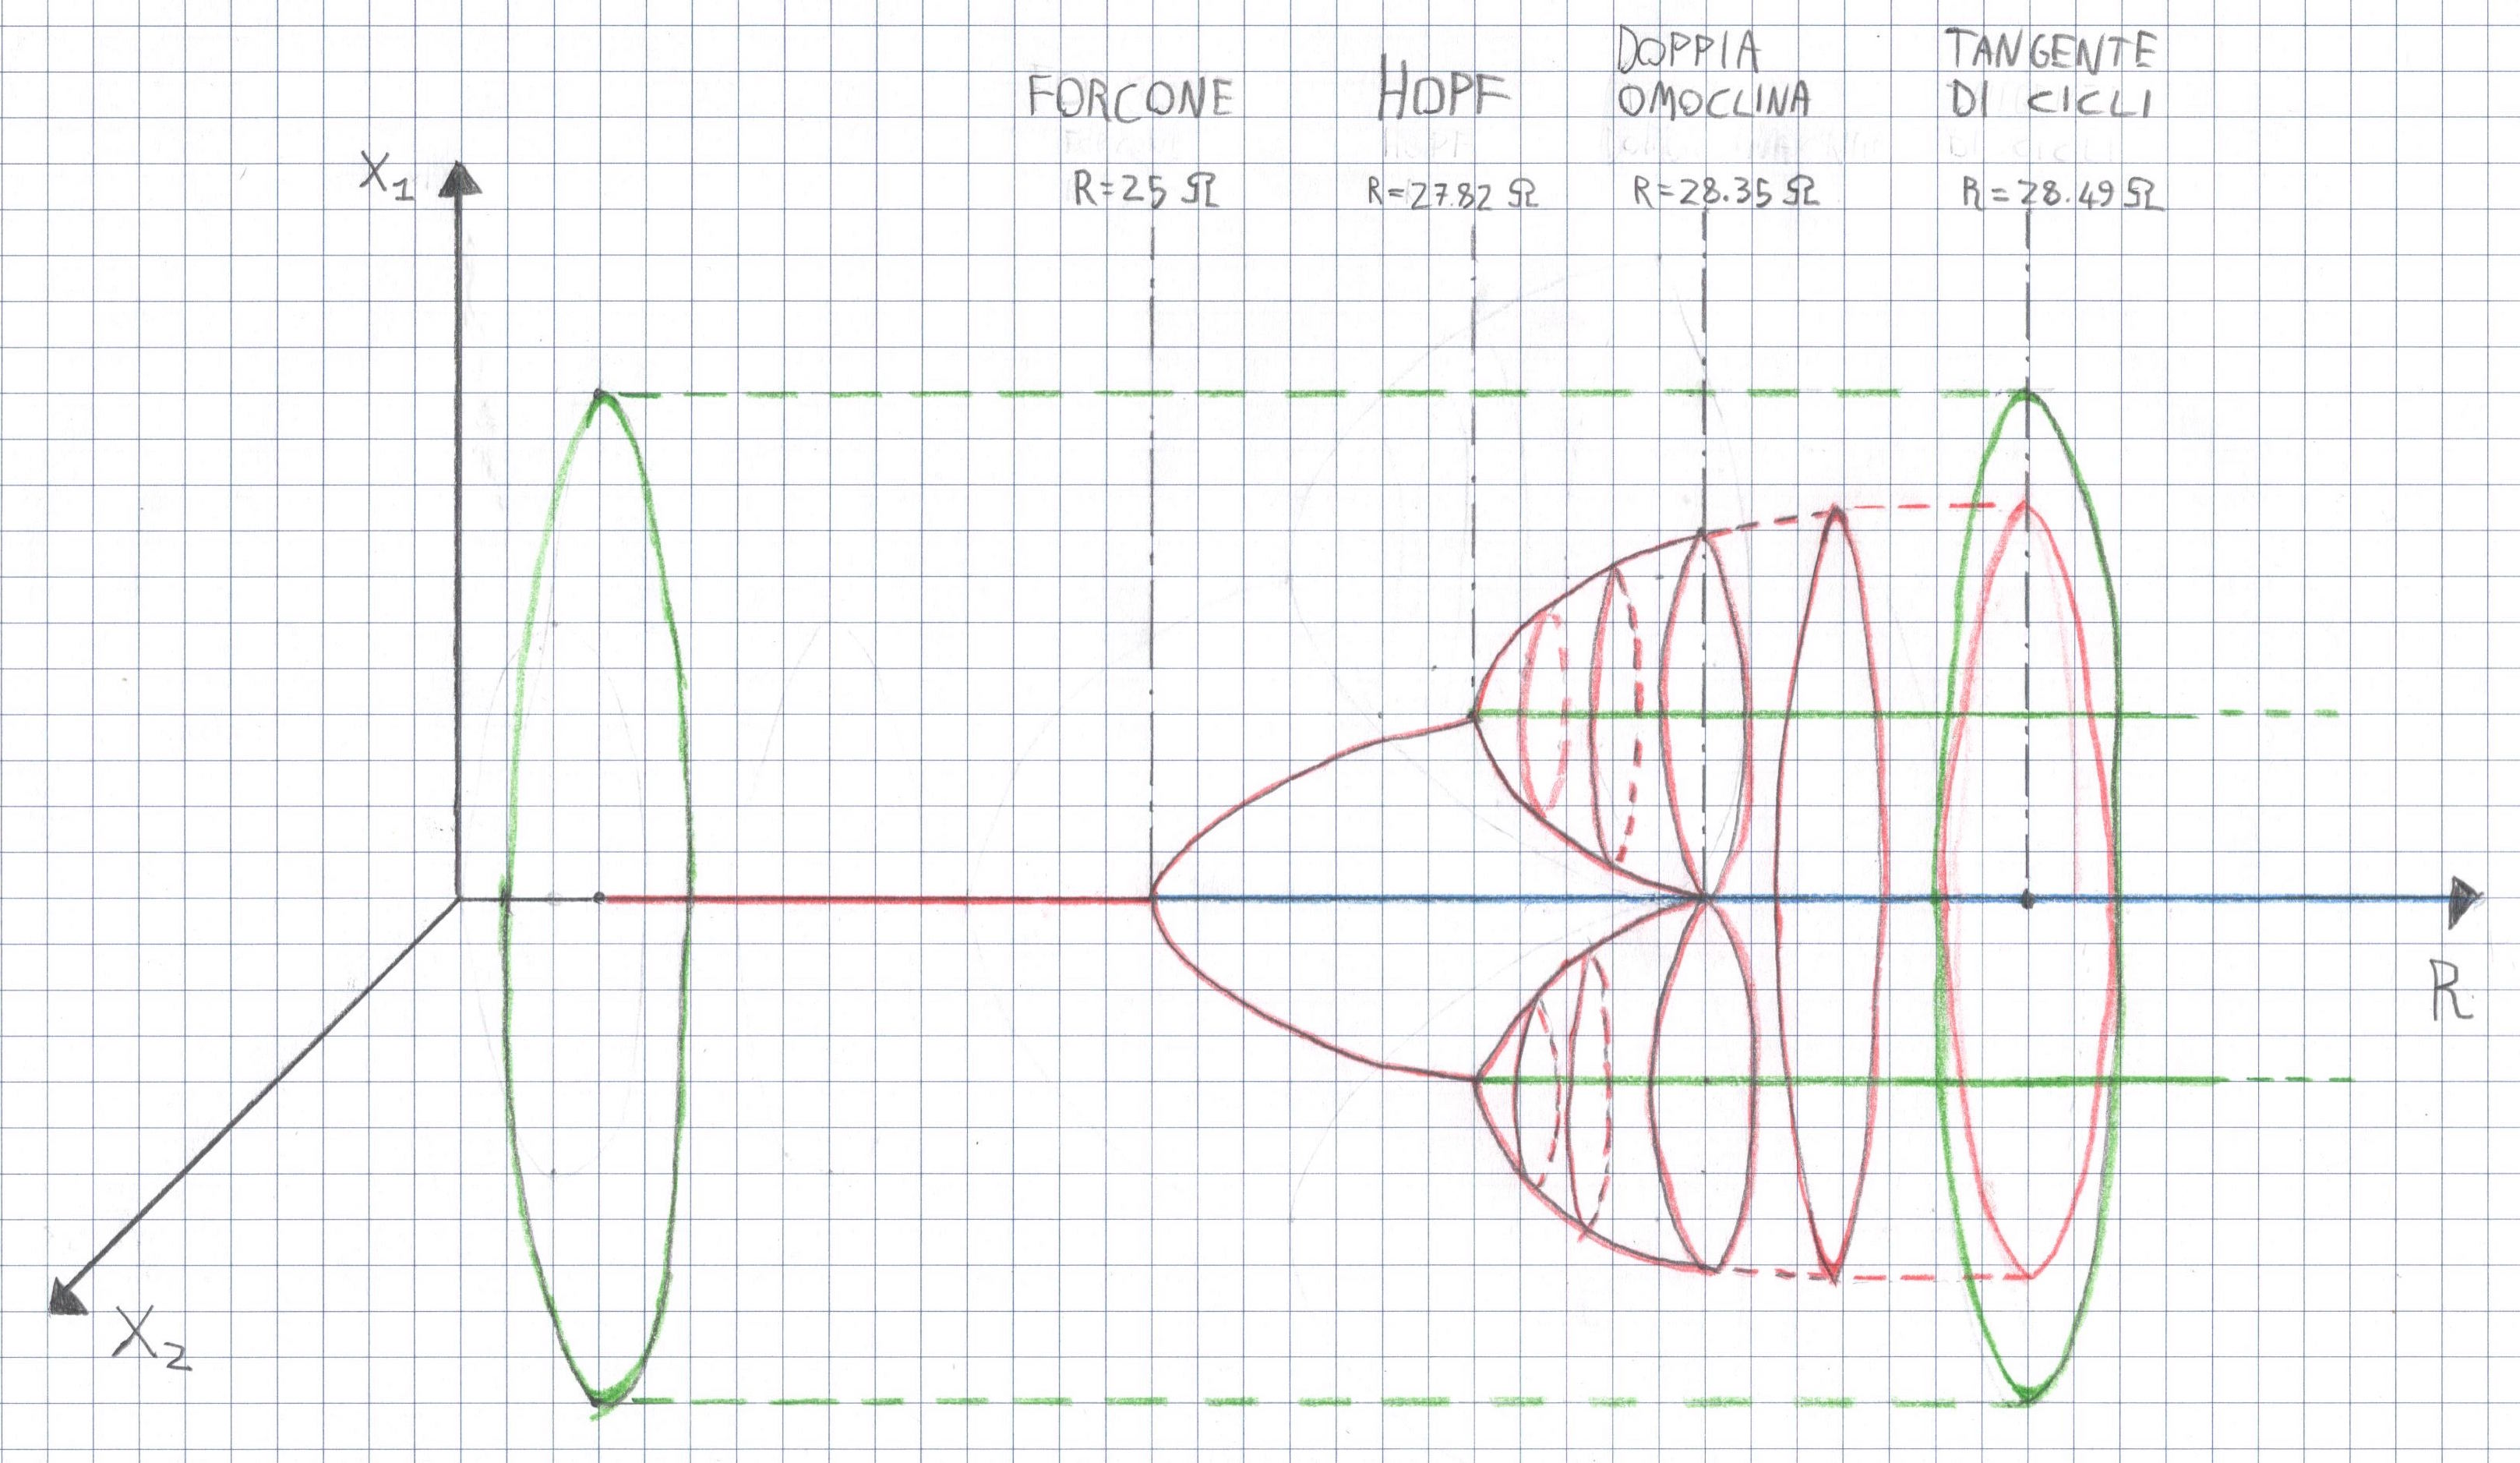
\includegraphics[width=\textwidth]{images/diagramma_qualitativo}
\caption{Il diagramma qualitativo delle biforcazioni in funzione di $R$.}
\label{fig:biforcazioni-qualitativo}
\end{figure}

\begin{figure}
\centering
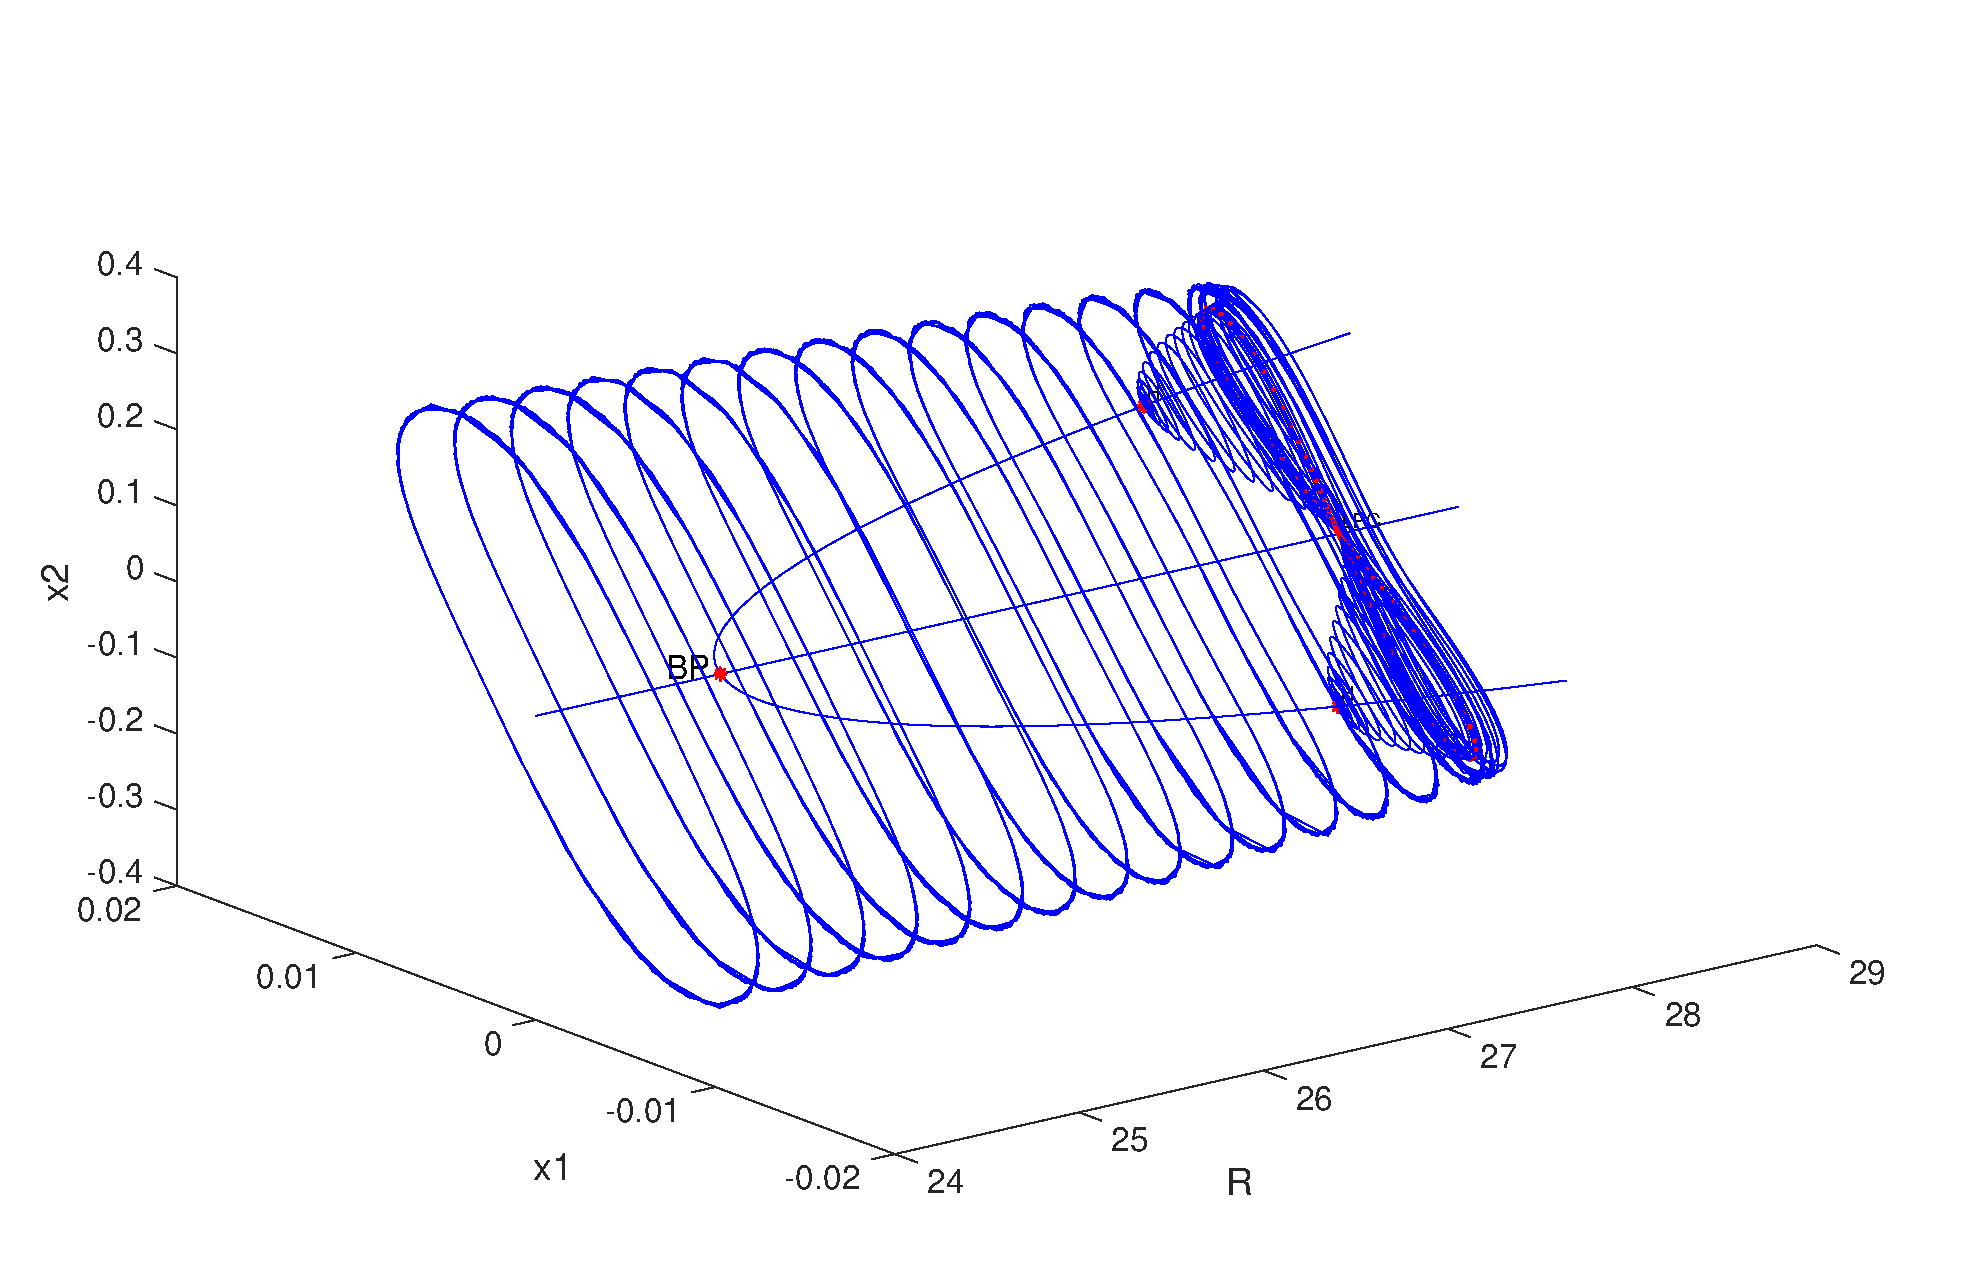
\includegraphics[width=0.8\textwidth]{matcont/BiforcazioniCompleto}
\caption{Il diagramma delle biforcazioni in funzione di $R$.}
\label{fig:biforcazioni-matcont}
\end{figure}
